%!TEX root =  ../main.tex

\subsection{STATS in the TI}

\objective{Create appropriate regressions of data in a grapher.}


In order to proceed from numerical to algebraic and graphical models of
real-world situations, we need to perform \textbf{regression analysis}, a thoughtful
process of establishing the strength and kind of relationship between two
variables.  The entirety of Chapter 13 is about regression.
For now, we simply seek to make equations from sets of ordered pairs.
\index{regression}

\index{TI-8*!data entry}
Your TI-8* has \emph{some} capacity as a spreadsheet.  You may entered tabular data, 
graph, and analyze the results on this little computer!  Most things you will need start by
pressing the \Touche[style=function,principal={STAT}] button.
This information is stored in lists, like \texttt{L$_1$}, \texttt{L$_2$}, \texttt{L$_3$}, etc.  
These names are not letters found with the \Touche[style=function,principal={\small ALPHA}]
button, but whole characters.  They can be accessed via \Touche[style=function,principal={2ND}]
\Touche[style=number, principal=1], \Touche[style=function,principal={2ND}] 
\Touche[style=number, principal=2], etc.  The most normal way to proceed is to put $x$ 
data in \texttt{L$_1$} and $y$'s in \texttt{L$_2$}.


Next, in order to make data you've entered visible, one must turn on a \texttt{STAT PLOT}.
This is done via \Touche[style=function,principal=2ND] \Touche[style=function,principal=Y=].
Here you will see three different \texttt{STAT PLOT}s you can turn on or off.  Press
\Touche[style=function,principal={\small ENTER}] to select 1, and then again to turn it on.
Be sure to turn \texttt{STAT PLOT}s off when you're not using them, so as not to obfuscate
other graphs.


\subsubsection{Windows}\index{TI-8*!window}
One of the trickier things to manage on the TI-8* is the \texttt{WINDOW}.  The Cartesian plane is 
a big place, and finding your place in it can be harder stilld.  Having a grasp
on concepts like domain and range is once again worth it's weight in gold.

First of all, the TI-8* does try to help you out by offering several automatic options, which 
may or may not be  useful.  The most commonly used is \Touche[style=function,principal=ZOOM]
\Touche[style=number, principal=6]: \texttt{ZStandard}.  This is the common window, 
$-10\le x\le 10$ and $-10\le y\le 10$, with tick-marks every unit.  When in doubt, start here.

If, however, the data is given to you, make the \texttt{Xmin} the smallest element in the domain,
and \texttt{Xmax} the biggest (press WINDOW).  Similarly, the range should dictate your \texttt{Ymin} and 
\texttt{Ymax}.  For truly useful graphs, determine the breadth of both the domain and range, 
by subtracting the smallest element from the biggest.  Divide these by 20 and you will get
the \texttt{Xscl} and \texttt{Yscl} respectively (the little tick marks).

Of course, the procedure outlined in the last paragraph will not work for most function definitions,
since they will go on forever, often in both domain and range.  This means you just have to know
what are the salient features of a given kind of graph, and how to bring them into view.  For example,
a quadratic function's most important point the vertex, the place where it changes from increasing
to decreasing or visa versa.  Most of the time, this is involves a process of guess-and-check,
combined with every-honing instincts.

\subsubsection{Table}\index{TI-8*!table}
\Touche[style=function,principal=2ND] \Touche[style=function,principal={\small GRAPH}] is
the very helpful \texttt{TABLE} of data.  This is especially useful at comparing multiple functions on 
the same inputs.  The default to start at $x=1$ and increment by one from there on up.
To customize the table, you must press \Touche[style=function,principal=2ND] 
\Touche[style=function,principal={WIND}], which is called \texttt{TABLESETUP}.  
You can either make the table 
automatically increment through the domain, starting where you wish and skipping by the
same amount every time (\texttt{AUTO}), or you can manually enter values for the input (
\texttt{Ask}).


\paragraph{Linear Regression}
In you are given only two points and told to make a line through them both, then the problem is 
very easy system of two equations, and can be immediately solved via the RREF of a 2x3 matrix.
However, most scientific and real-life data is ``fuzzy'', and no line can go through all the data points.
In such situations, it is best to enter all the data and let the machines find the ``line of best fit''.  In 
simple cases, it is simply a matter of constructing the line where half the data is below and half is 
above.  But as data multiplies, this becomes harder and harder.\index{regression!linear}

\begin{example}[Linear Regression]
Find the line of best fit for the data in this table.

\begin{tabular}{c|c}
   \textbf{x} & \textbf{y} \\ \hline 
   1 & 1 \\
   2 & 2 \\
   3 & 1.3 \\
   4 & 3.75 \\
   5 & 2.25 \\
\end{tabular}

\paragraph{Solution}
Using a TI-8*, press STAT, EDIT, and enter the $x$ data in $L_1$ and the $y$ data in $L_2$.  If
there is already data clogging up these lists, move up to their names at the top of the window
and press CLEAR, then ENTER.  Assuming
the appropriate STATPLOT is on, press ZOOM 9 and inspect the graph.  It is not a simple linear graph, where
any line passing through any two of the points is perfect, so we proceed with the calculator regression

Pressing STAT, moving over to CALC, we scroll down to LINREG(AX+B).  Depending upon your version,
you may need to type $L_1, L_2, Y_1$ or select all these setting for a menu.  ($Y_1$ is located under
VARS, Y-VARS, FUNCTION... and should be entered under `Store EQ'.) Press ENTER or CALCULATE 
and the answer of $y=.425x+.785$ appears, as well as the coefficient of determination $r^2$.  (If your
calculator doesn't show you $r^2$, you might need to press CATALOG, scroll down to DiagnosticOn
and turn it on.). We will learn about $r$ and $r^2$ in 13.3, but for now it is enough to say it is helpful
measure of how closely the equation ``hugs'' the data.

Finally, press GRAPH to see the equation against the data.
\end{example}

\paragraph{Quadratic Regression}\index{regression!quadratic}
When the data rise and falls (or falls and rises), it is possible that a quadratic equation would be a better fit.
Visualize the data and then consider running QuadReg and generating an equation of the form $ax^2+bx+c$.
Perfect data can be solved simply with a 3x4 matrix.

\paragraph{Exponential and Logarithmic Regression}\index{regression!exponential}
ExpReg and LnReg are great tools, if you know how to choose between them.

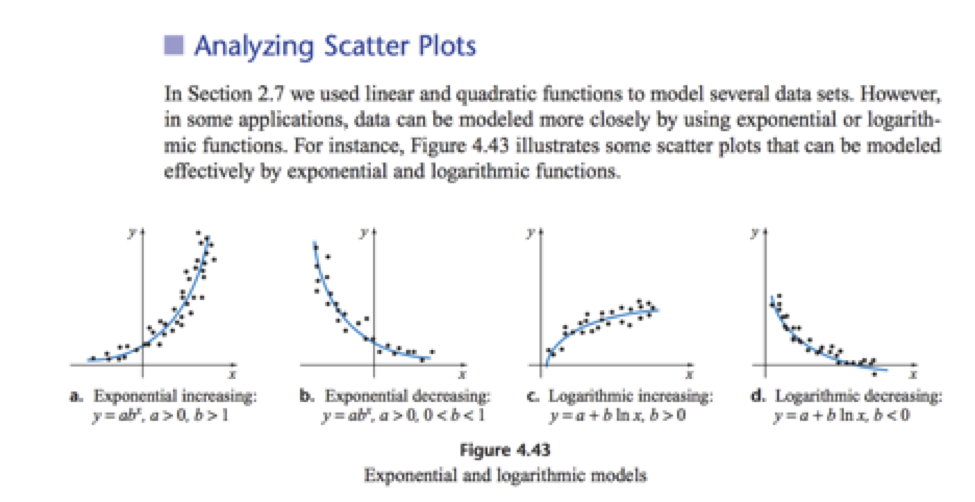
\includegraphics[scale=0.8]{expln.png}\index{regression!logarithmic}

Exponential functions have a horizontal asymptote at $y=0$ if un-translated.  Logarithmic functions
has a vertical asymptote at $x=0$ if un-translated.  Most practical situations, it is always possible to tell if
there is a limiting $x$ or $y$ value.  If there are multiple asymptotes, it is probably a power function.

\paragraph{Sinusoidal Regression}\index{regression!sinusoidal}
While we have not formally introduced period functions yet, it is relatively easy to run a SinReg in the calculator
and get an equation from data.  The only additional questions you must answer are the number of iterations ---
how many times should the calculator pour over the data (the max is 16, which you should use for all ``fuzzy''
data) --- and the \textbf{period} --- the distance from peak to peak, or trough to trough.  For now, the period will
always be given to you.
